\documentclass{article}

\usepackage[italian]{babel}
\usepackage[margin=2cm, footskip=5mm]{geometry}
% questi package non sono necessari in lualatex; ref https://tex.stackexchange.com/a/413046
% \usepackage[utf8]{inputenc}
% \usepackage[T1]{fontenc}
\usepackage{enumitem}
\usepackage{hyperref}
\usepackage{titlesec}
\usepackage{soulutf8}
\usepackage{contour}
\usepackage{float}
\usepackage{graphicx}
\usepackage{fancyhdr}
\usepackage{longtable}
\usepackage[table]{xcolor}
\usepackage{titling}
\usepackage{lastpage}
\usepackage{ifthen}
\usepackage{calc}
\usepackage{minted}
\usepackage{pgfgantt}
\usepackage{subfiles}

\newlength{\imgwidth}

\newcommand\scalegraphics[1]{%
    \settowidth{\imgwidth}{\includegraphics{#1}}%
    \setlength{\imgwidth}{\minof{\imgwidth}{\textwidth}}%
    \includegraphics[width=\imgwidth]{#1}%
}

% XXX definizione dei percorsi in cui cercare immagini
\graphicspath{ {./}
    {./img/}
}

% esempio di utilizzo: \appendToGraphicspath{./img/} (un comando diverso per ogni path da includere)
% N.B.: ci DEVE essere un forward slash alla fine del path, a indicare che è una cartella.
\makeatletter
\newcommand\appendToGraphicspath[1]{%
  \g@addto@macro\Ginput@path{{#1}}%
}
\makeatother

% setup della sottolineatura
\setuldepth{Flat}
\contourlength{0.8pt}

\newcommand{\uline}[1]{%
  \ul{{\phantom{#1}}}%
  \llap{\contour{white}{#1}}%
}

% setup dei link
\hypersetup{
  colorlinks=true, % set true if you want colored links
  linktoc=all,     % set to all if you want both sections and subsections linked
  linkcolor=black, % choose some color if you want links to stand out
}

% setup di header e footer
\pagestyle{fancy}

\fancyhf{}
\fancyhead[L]{\includegraphics[width=1cm]{logo.png}}
\fancyhead[R]{\thetitle}
\fancyfoot[R]{\thepage\ di~\pageref{LastPage}}

\fancypagestyle{nopage}{%
  \fancyfoot{}%
}

\setlength{\headheight}{1.2cm}

% setup forma \paragraph e \subparagraph
\titleformat{\paragraph}[hang]{\normalfont\normalsize\bfseries}{\theparagraph}{1em}{}
\titleformat{\subparagraph}[hang]{\normalfont\normalsize\bfseries}{\thesubparagraph}{1em}{}

% setup profondità indice di default
\setcounter{secnumdepth}{5}
\setcounter{tocdepth}{5}

% shortcut per i placeholder
\newcommand{\plchold}[1]{\textit{\{#1\}}} % chktex 20

% hook per lo script che genera il glossario
\newcommand{\glossario}[1]{\underline{#1}\textsubscript{g}}

% definizione dei comandi \uso e \stato
\makeatletter
\newcommand{\setUso}[1]{%
  \newcommand{\@uso}{#1}%
}
\newcommand{\uso}{\@uso}

\newcommand{\setStato}[1]{%
  \newcommand{\@stato}{#1}%
}
\newcommand{\stato}{\@stato}

\newcommand{\setVersione}[1]{%
  \newcommand{\@versione}{#1}%
}
\newcommand{\versione}{\@versione}

\newcommand{\setResponsabile}[1]{%
  \newcommand{\@responsabile}{#1}%
}
\newcommand{\responsabile}{\@responsabile}

\newcommand{\setRedattori}[1]{%
  \newcommand{\@redattori}{#1}%
}
\newcommand{\redattori}{\@redattori}

\newcommand{\setVerificatori}[1]{%
  \newcommand{\@verificatori}{#1}%
}
\newcommand{\verificatori}{\@verificatori}

\newcommand{\setDescrizione}[1]{%
  \newcommand{\@descrizione}{#1}%
}
\newcommand{\descrizione}{\@descrizione}

\newcommand{\setModifiche}[1]{%
  \newcommand{\@modifiche}{#1}%
}

\newcommand{\modifiche}{\@modifiche}

\makeatother

% setup delle description
\setlist[description,1]{font=$\bullet$\hspace{1.5mm}, labelwidth=* leftmargin=*,labelindent=12.5mm}
\setlist[description,2]{font=$\bullet$\hspace{1.5mm}, leftmargin=*,labelindent=12.5mm}
\appendToGraphicspath{../../commons/img/}

\title{Verbale esterno --- 02/03/2020}

\setResponsabile{Riccardo Agatea}
\setRedattori{Luca Ercole}
\setVerificatori{
  Alberto Gobbo \\ &
  Fabio Scettro
}
\setUso{Esterno}
\setDescrizione{Verbale dell'incontro di GruppOne del 02/03/2020}
\setModifiche{%
\cellcolor{white!80!lightgray!100} & Riccardo Agatea & 2020--03--03 & approva documento \\%
\cellcolor{white!80!lightgray!100} & Verificatori & 2020--03--03 & verifica verbale \\%
\cellcolor{white!80!lightgray!100} & Luca Ercole & 2020--03--02 & stendi verbale %
}

\disabilitaVersione{}
\disabilitaElencoFigure{}
\disabilitaElencoTabelle{}

\begin{document}

\thispagestyle{empty}
\pagenumbering{gobble}

\begin{center}

  \includegraphics[width=8.5cm]{\commons/img/logo.png}\\
  {\Large GruppOne - progetto "Stalker"}\\
  \vspace{1.5cm}

  {\Huge \thetitle}
  \vspace{1.5cm}

  \begin{table}[H]
    \centering

    \begin{tabular}{r|l}
      \textbf{Versione}     & \versione              \\
      \textbf{Approvazione} & \responsabile          \\
      \textbf{Redazione}    & \redattori             \\
      \textbf{Verifica}     & \verificatori          \\
      \textbf{Stato}        & \stato                 \\
      \textbf{Uso}          & \uso                   \\
      \textbf{Destinato a}  & Imola Informatica      \\
                            & GruppOne               \\
                            & Prof. Tullio Vardanega \\
                            & Prof. Riccardo Cardin  \\
    \end{tabular}
  \end{table}

  \vspace{3cm}
  \textbf{Descrizione}\\
  \descrizione\\
  \vfill
  \verb|gruppone.swe@gmail.com|
\end{center}

\newpage
\thispagestyle{nopage}

\section*{Registro delle modifiche}
\label{sec:registro_delle_modifiche}

\begin{table}[H]
  \label{tab:registro_delle_modifiche}

  \centering
  \rowcolors{2}{lightgray}{white!80!lightgray!100}

  \begin{longtable}[c]{c c c c l}
    \rowcolor{darkgray!90!}\color{white}{\textbf{Versione}} & \color{white}{\textbf{Data}} & \color{white}{\textbf{Nominativo}} & \color{white}{\textbf{Ruolo}} & \color{white}{\textbf{Descrizione}} \\\endhead
    \modifiche
  \end{longtable}
\end{table}

% section registro_delle_modifiche (end)
\newpage

\thispagestyle{nopage}
\pagenumbering{roman}
\tableofcontents

\newpage

\pagenumbering{arabic}


\section{Informazioni logistiche}%
\label{sec:informazioni_logistiche}

\begin{description}
  \item [Luogo] chiamata Hangouts
  \item [Data] 02/03/2020
  \item [Ora] 18:00 \symbol{8594} 19:00
\end{description}

\subsection{Membri del gruppo presenti}%
\label{sub:membri_del_gruppo_presenti}

\begin{enumerate}
  \item Riccardo Agatea
  % \item Tobia Apolloni
  \item Riccardo Cestaro
  % \item Alberto Cocco
  \item Luca Ercole
  \item Alberto Gobbo
  \item Alessandro Rizzo
  % \item Fabio Scettro
\end{enumerate}

% sub:membri_del_gruppo_presenti (end)

\subsection{Altri partecipanti}%
\label{sub:altri_partecipanti}

\begin{enumerate}
  \item Davide Zanetti (Imola Informatica, proponente del capitolato)
\end{enumerate}

% sub:altri_partecipanti (end)
% sec:informazioni_logistiche (end)

\section{Introduzione}%
\label{sec:introduzione}

L'incontro è avvenuto tramite chiamata Hangouts.
Lo scopo principale era di discutere e finalizzare le nostre scelte tecnologiche per il progetto.

\section{Ordine del giorno}%
\label{sec:ordine_del_giorno}

\begin{itemize}
  \item Conversazione Telegram
  \item Tecnologie frontend
  \item Tecnologie backend
  \item Accesso a server di Imola Informatica
\end{itemize}

\section{Conversazione Telegram}%
\label{sec:conversazione_telegram}

Riportiamo per completezza la conversazione avvenuta su telegram:

\begin{enumerate}
  \item Secondo te è una scelta valida utilizzare i framework NativeScript/Angular per riutilizzare codice tra le applicazioni web e mobile?
  \item Hai consigli per il framework Java da utilizzare? Stiamo guardando Quarkus e Spring Boot o Spring Data, ma non avendo esperienza facciamo fatica a valutare quale sia più adatto e/o semplice da utilizzare.
\end{enumerate}

A cui il proponente ha risposto:

\begin{enumerate}
  \item Non sono molto pratico di questo ad essere onesto, provo ad informarmi con qualche collega più esperto e vedo di trovarvi una risposta sensata.
  \item Personalmente conosco bene Spring Boot e Spring Data (molto più diffusi negli ambienti dove lavoro), sono un po' più carente per quanto riguarda Quarkus (che comunque mi sembra interessante come framework).
        Quindi, validi entrambi, sul primo posso aiutarvi più facilmente ed è abbastanza facile da usare, sul secondo non sono molto esperto ma se volete provarlo mi documento con voi.
\end{enumerate}

% sec:conversazione_telegram (end)

\section{Tecnologie frontend}%
\label{sec:tecnologie_frontend}

Il proponente ci ha fatto presente che utilizzare NativeScript non è una soluzione particolarmente pulita perché in caso di difficoltà si deve ricadere sulla scrittura di classi in Java puro;
quindi il vantaggio di utilizzarlo probabilmente non vale il rischio di incontrare problemi difficilmente risolvibili più avanti nello sviluppo.

L'aspetto di riutilizzo del codice tra web/mobile è un bonus, ma l'applicazione che stiamo progettando è abbastanza contenuta quindi ha consigliato di fare tutto in Java.

Inoltre, integrare mappe nell'applicazione mobile (ad es.\ nelle schermate delle organizzazioni) dovrebbe essere semplice.

L'applicazione deve funzionare perlomeno su Android 9, ma comunque faremo riferimento alla \href{https://developer.android.com/distribute/best-practices/develop/target-sdk}{guida ufficiale}

\subsection{Geofences}%
\label{sub:geofences}

Il proponente ha confermato la validità della nostra idea di utilizzare le geofences come confine esterno centrato sui luoghi delle organizzazioni.
In particolare, le potremmo utilizzare per garantire che un utente è uscito da un luogo (il proponente ha usato il termine ``rollback'').

Inoltre, possiamo farci affidamento per diminuire il consumo energetico dell'applicazione quando gli utenti sono lontani dalle organizzazioni.

% sec:tecnologie_frontend (end)

\subsection{Applicazione web}%
\label{sub:applicazione_web}

A prescindere dalle tecnologie utilizzate per l'applicazione mobile, usiamo il framework Angular per l'applicazione web.

Il proponente ci ha consigliato \href{https://www.selenium.dev/}{Selenium} per testarne gli aspetti grafici.

% sub:applicazione_web (end)

\section{Tecnologie backend}%
\label{sec:tecnologie_lato_server}

Spring Boot è estremamente diffuso e ha un ecosistema molto grande, quindi è probabilmente utile per noi imparare a utilizzarlo.

Il proponente ha menzionato il modulo \href{https://docs.spring.io/spring/docs/current/spring-framework-reference/web-reactive.html}{WebFlux} che permette di utilizzare il paradigma del Reactive Programming.

Per quanto riguarda le funzionalità LDAP, Davide ha detto che possiamo utilizzare Spring LDAP (una libreria del framework), ma che molto probabilmente è sufficiente utilizzare un'API RESTful.
Ha menzionato in particolare la \href{https://directory.fedoraproject.org/docs/389ds/design/ldap-rest-api.html}{389 Directory Server RESTful API}

\subsection{Progettazione API}%
\label{sub:progettazione_api}

Il proponente ci ha consigliato di guardare la risorsa \href{https://opensource.zalando.com/restful-api-guidelines/}{Zalando RESTful API and Event Scheme Guidelines}.

Inoltre ha detto che non consiglia di utilizzare gli strumenti di generazione automatica del codice di Swagger, perché la qualità del codice generato è molto bassa.

% sub:progettazione_api (end)
\subsection{Containerization}%
\label{sub:containerization}

Il proponente ci ha consigliato di concentrarci prima sull'aspetto di ``containerizzazione'' attraverso Docker, perché se viene fatto bene rende molto semplice agganciare a posteriori i pod di Kubernetes per la gestione e scalabilità dell'applicativo.

Si è anche raccomandato di fare molto affidamento sulle immagini ufficiali di software disponibili su Docker Hub (come ad es.\ i database SQL), perché semplificano enormemente la configurazione dei servizi.

% sub:containerization (end)

% sec:tecnologie_lato_server (end)

\section{Accesso a server di Imola Informatica}%
\label{sec:accesso_a_server_di_imola_informatica}

Nei prossimi giorni entreremo in contatto via email con un tecnico di Imola Informatica che ci creerà un'utenza sulle macchine del loro laboratorio.

Il proponente ci ha fatto presente che non dobbiamo salvare dati persistenti sul loro server, perché spesso le macchine vengono resettate.

% sec:accesso_a_server_di_imola_informatica (end)

\newpage
\section{Registro delle decisioni}%
\label{sec:registro_delle_decisioni}

\begin{description}
  \item[20200302-ext-001] Usare Spring Boot e Spring LDAP per il backend.
  \item[20200302-ext-002] Progettare prima l'API in maniera da avere un approccio \textit{Contract First}.
  \item[20200302-ext-003] Usare MySQL per i dati più persistenti.
  \item[20200302-ext-004] Usare InfluxDB per le serie temporali (in part.\ presenza/assenza degli utenti nei luoghi).
  \item[20200302-ext-005] Posticipare la decisione sulle tecnologie frontend a dopo la finalizzazione dell'API\@.
\end{description}

\end{document}
